\subsection{Gantt chart deel 1} 
	\begin{figure}[H]
		\begin{center}
			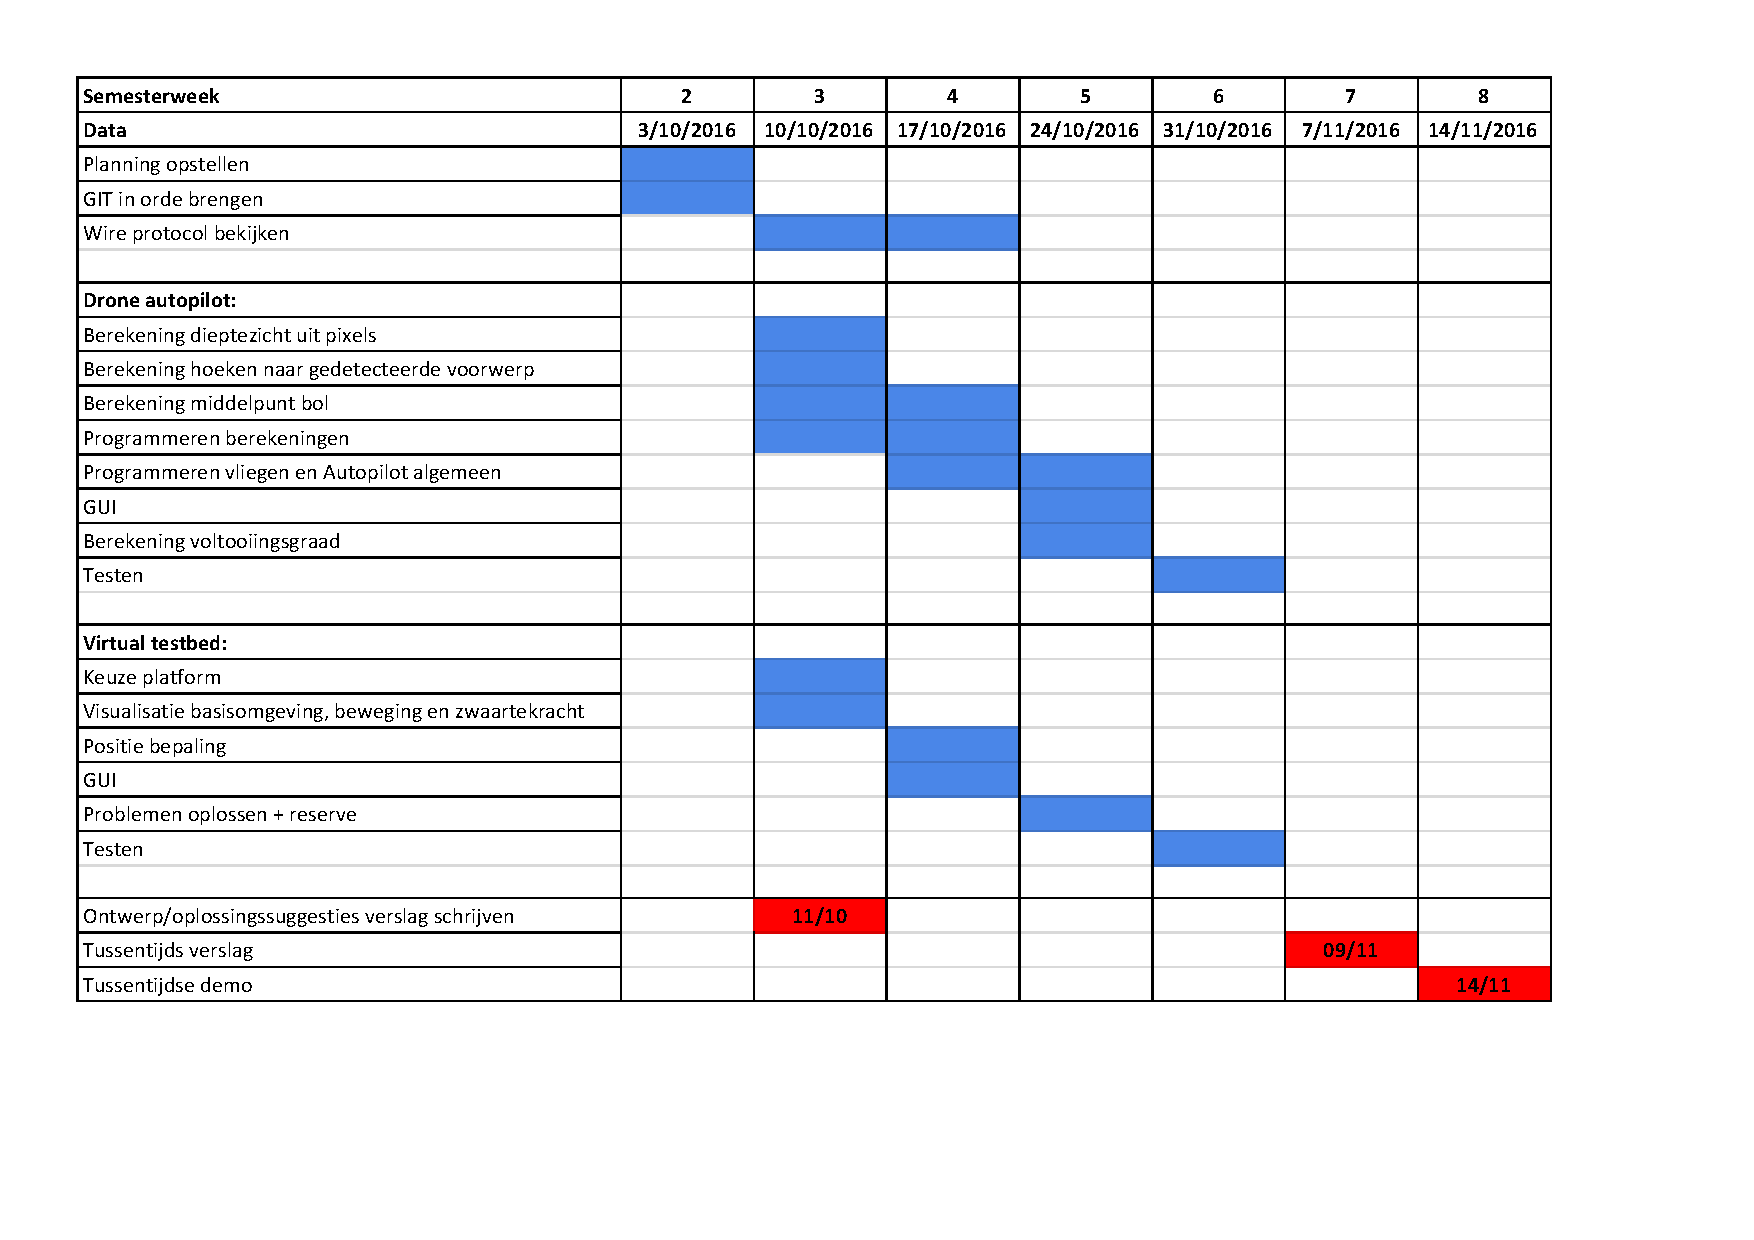
\includegraphics[scale=0.60]{Planning_Deel1.pdf}
		\end{center}
		\caption{Deze Gantt chart geeft de planning gedetailleerd weer van het eerste deel. De verschillende delen van de mijlpalen worden opgesplitst om een gedetailleerde taakverdeling te kunnen maken. De deadlines worden in het rood aangeduid.}
	\end{figure}
\subsection{Gantt chart deel 2} 
	\begin{figure}[H]
		\begin{center}
			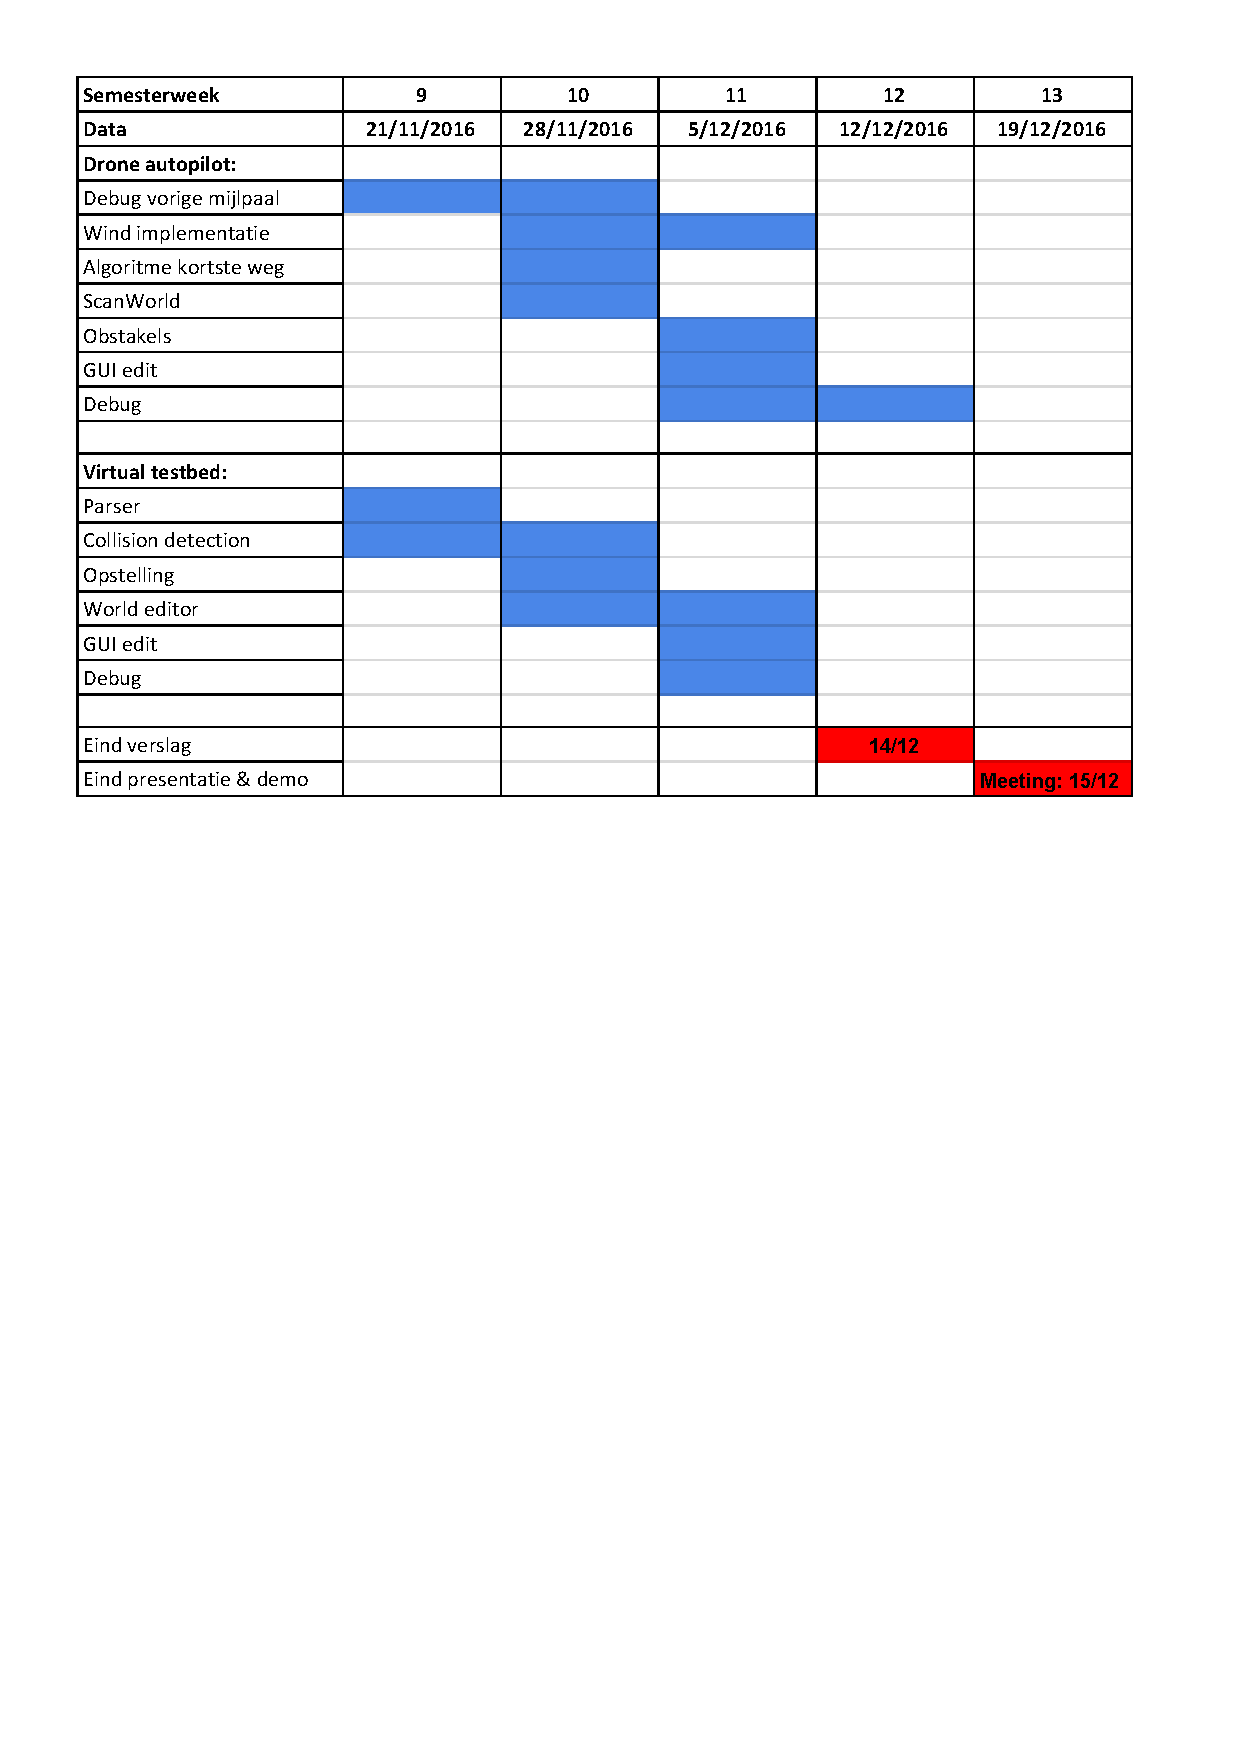
\includegraphics[scale=0.65]{Planning_Deel2.pdf}
		\end{center}
		\caption{Deze Gantt chart geeft de planning gedetailleerd weer van het tweede deel. De verschillende delen van de mijlpalen worden opgesplitst om een gedetailleerde taakverdeling te kunnen maken. Ook wordt er tijd voorzien om de tekorten van vorige mijlpalen in te halen. De deadlines worden in het rood aangeduid.}
	\end{figure}